\documentclass[tikz, border=20pt]{standalone}
\usepackage[utf8]{inputenc}
\usepackage{helvet}
\renewcommand{\familydefault}{\sfdefault}
\usetikzlibrary{positioning, shapes.geometric, arrows.meta, calc, backgrounds}

\begin{document}
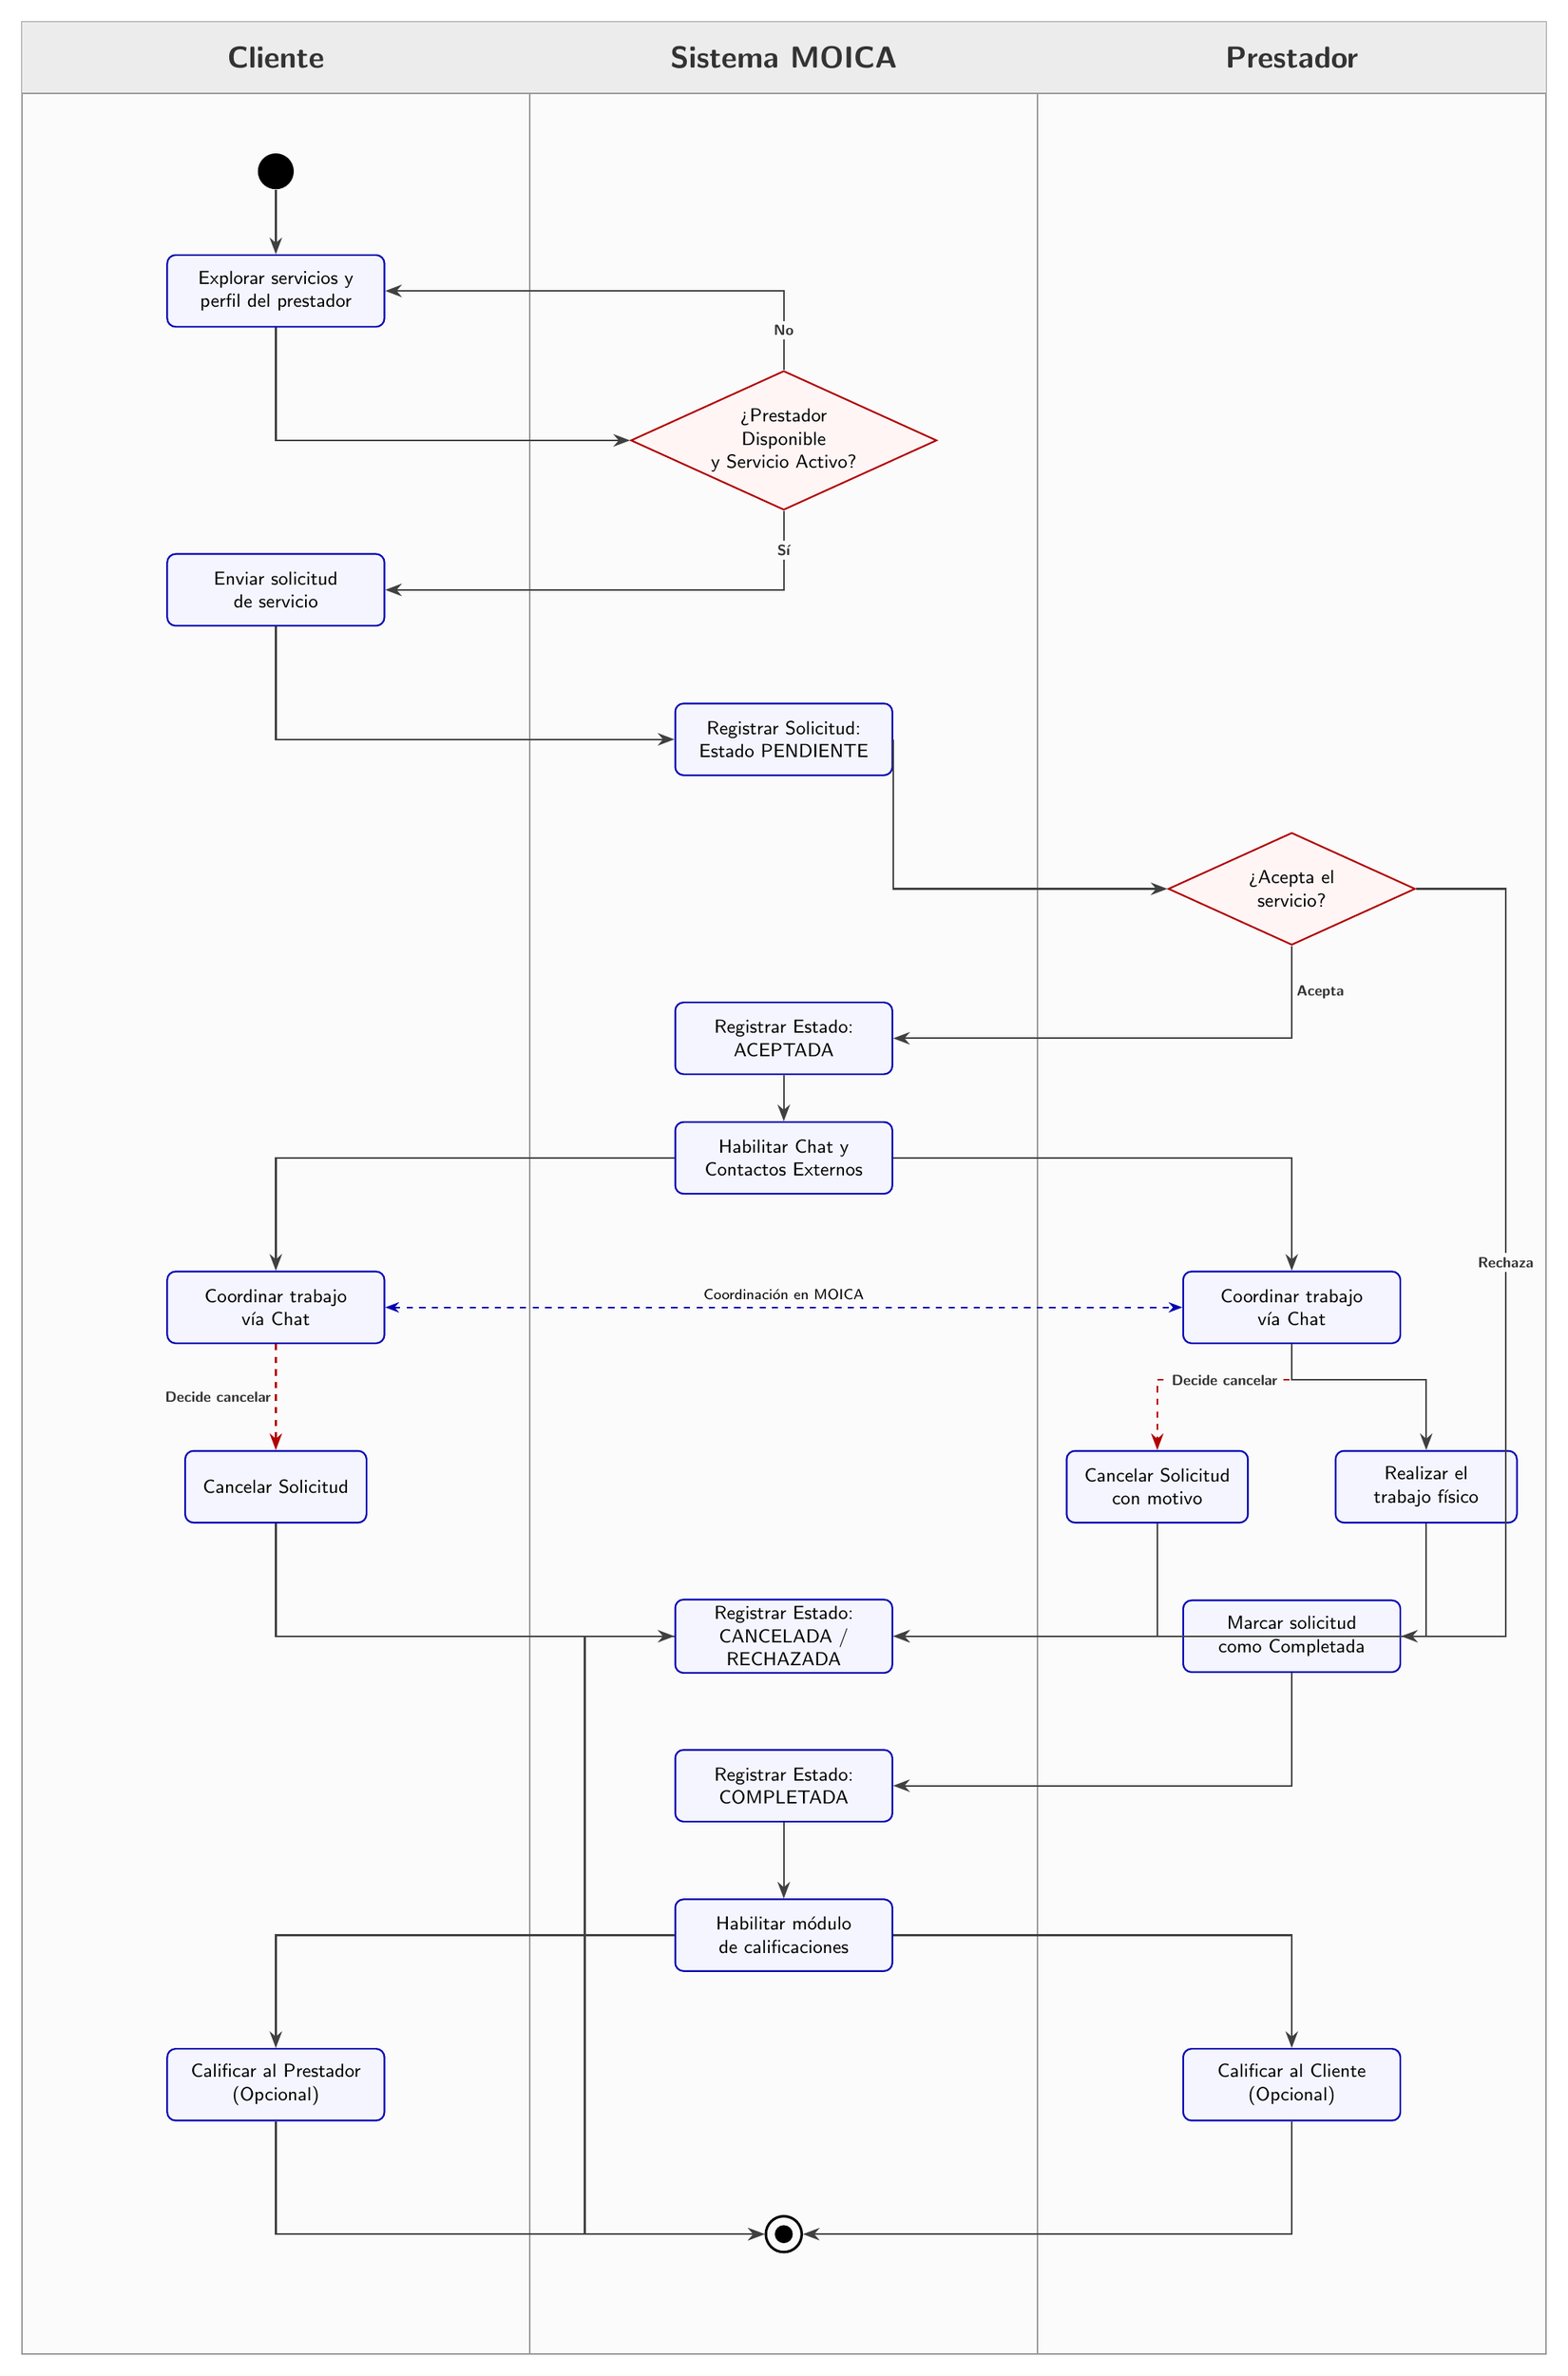
\begin{tikzpicture}[
    % ====================
    % ESTILOS DE NODOS
    % ====================
    action/.style={
        rectangle, rounded corners=4pt, 
        draw=blue!70!black, fill=blue!4, thick, 
        align=center, font=\small\sffamily, 
        minimum height=1.2cm, text width=3.4cm
    },
    decision/.style={
        diamond, aspect=2.2, 
        draw=red!70!black, fill=red!4, thick, 
        align=center, font=\small\sffamily, 
        text width=2.8cm, inner sep=0pt
    },
    start/.style={
        circle, fill=black, 
        minimum size=0.6cm, inner sep=0pt
    },
    end/.style={
        circle, draw=black, very thick, 
        minimum size=0.6cm, inner sep=0pt,
        path picture={
            \fill (path picture bounding box.center) circle (0.15cm);
        }
    },
    line/.style={
        thick, draw=black!75, -{Stealth[scale=1.2]}
    },
    label_style/.style={
        fill=gray!3, inner sep=2pt, font=\scriptsize\bfseries\sffamily, text=black!80
    }
]

% ====================
% FONDOS Y CARRILES (SWIMLANES)
% ====================
\pgfdeclarelayer{background}
\pgfsetlayers{background,main}

\begin{pgfonlayer}{background}
    % Fondo general
    \fill[gray!3] (0, 0) rectangle (25.5, -39);
    
    % Bordes exteriores
    \draw[thick, black!40] (0, 0) rectangle (25.5, -39);
    
    % Líneas divisorias de carriles (8.5cm por columna)
    \draw[thick, black!40] (8.5, 0) -- (8.5, -39);
    \draw[thick, black!40] (17, 0) -- (17, -39);

    % Cabeceras de carriles
    \fill[gray!15] (0, 0) rectangle (8.5, -1.2);
    \node[font=\Large\sffamily\bfseries, text=black!80] at (4.25, -0.6) {Cliente};

    \fill[gray!15] (8.5, 0) rectangle (17, -1.2);
    \node[font=\Large\sffamily\bfseries, text=black!80] at (12.75, -0.6) {Sistema MOICA};

    \fill[gray!15] (17, 0) rectangle (25.5, -1.2);
    \node[font=\Large\sffamily\bfseries, text=black!80] at (21.25, -0.6) {Prestador};

    % Línea inferior de las cabeceras
    \draw[thick, black!40] (0, -1.2) -- (25.5, -1.2);
\end{pgfonlayer}

% ====================
% DEFINICIÓN DE NODOS
% ====================

% Nodo de Inicio
\node[start] (start) at (4.25, -2.5) {};

% Nodos - Cliente (Columna 1: x = 4.25)
\node[action] (C1) at (4.25, -4.5) {Explorar servicios y\\perfil del prestador};
\node[action] (C2) at (4.25, -9.5) {Enviar solicitud\\de servicio};
\node[action] (C3) at (4.25, -21.5) {Coordinar trabajo\\vía Chat};
\node[action, text width=2.8cm] (C5) at (4.25, -24.5) {Cancelar Solicitud};
\node[action] (C4) at (4.25, -34.5) {Calificar al Prestador\\(Opcional)};

% Nodos - Sistema (Columna 2: x = 12.75)
\node[decision] (S1) at (12.75, -7) {¿Prestador Disponible\\y Servicio Activo?};
\node[action] (S2) at (12.75, -12) {Registrar Solicitud:\\Estado PENDIENTE};
\node[action] (S4) at (12.75, -17) {Registrar Estado:\\ACEPTADA};
\node[action] (S3) at (12.75, -19) {Habilitar Chat y\\Contactos Externos};
\node[action] (S5) at (12.75, -27) {Registrar Estado:\\CANCELADA / RECHAZADA};
\node[action] (S6) at (12.75, -29.5) {Registrar Estado:\\COMPLETADA};
\node[action] (S7) at (12.75, -32) {Habilitar módulo\\de calificaciones};

% Nodos - Prestador (Columna 3: x = 21.25 central, con desplazamientos)
\node[decision] (P1) at (21.25, -14.5) {¿Acepta el\\servicio?};
\node[action] (P2) at (21.25, -21.5) {Coordinar trabajo\\vía Chat};
\node[action, text width=2.8cm] (P6) at (19, -24.5) {Cancelar Solicitud\\con motivo};
\node[action, text width=2.8cm] (P3) at (23.5, -24.5) {Realizar el\\trabajo físico};
\node[action] (P4) at (21.25, -27) {Marcar solicitud\\como Completada};
\node[action] (P5) at (21.25, -34.5) {Calificar al Cliente\\(Opcional)};

% Nodo de Fin
\node[end] (end) at (12.75, -37) {};


% ====================
% RUTAS Y FLUJOS
% ====================

% Inicio a Explorar
\draw[line] (start) -- (C1);

% Explorar a Sistema
\draw[line] (C1.south) |- (S1.west);
\draw[line] (S1.north) |- node[pos=0.25, label_style] {No} (C1.east);
\draw[line] (S1.south) |- node[pos=0.25, label_style] {Sí} (C2.east);

% Enviar Solicitud a Sistema y Prestador
\draw[line] (C2.south) |- (S2.west);
\draw[line] (S2.east) |- (P1.west);

% Decisión del Prestador
\draw[line] (P1.south) |- node[pos=0.25, right, label_style] {Acepta} (S4.east);
% Ruta de rechazo (Bordea el carril derecho y baja hasta cancelar)
\draw[line] (P1.east) -- ++(1.5, 0) |- node[pos=0.25, label_style] {Rechaza} (S5.east);

% Proceso de Aceptación y Habilitación
\draw[line] (S4.south) -- (S3.north);
\draw[line] (S3.west) -| (C3.north);
\draw[line] (S3.east) -| (P2.north);

% Comunicación bidireccional
\draw[dashed, <->, >=Stealth, thick, draw=blue!70!black] 
    (C3.east) -- node[above, font=\scriptsize\sffamily, text=black] {Coordinación en MOICA} (P2.west);

% Caminos de Cancelación
\draw[line, dashed, draw=red!70!black] (C3.south) -- node[left, label_style] {Decide cancelar} (C5.north);
\draw[line, dashed, draw=red!70!black] (P2.south) -- ++(0, -0.6) -| node[pos=0.25, label_style] {Decide cancelar} (P6.north);
\draw[line] (C5.south) |- (S5.west);
\draw[line] (P6.south) |- (S5.east);

% Ruta de S5 a Fin (Baja evitando chocar con S6 y S7)
\draw[line] (S5.west) -- ++(-1.5, 0) |- (end.west);

% Continuación del Trabajo
\draw[line] (P2.south) -- ++(0, -0.6) -| (P3.north);
\draw[line] (P3.south) |- (P4.east);
\draw[line] (P4.south) |- (S6.east);
\draw[line] (S6.south) -- (S7.north);

% Calificaciones Finales
\draw[line] (S7.west) -| (C4.north);
\draw[line] (S7.east) -| (P5.north);

\draw[line] (C4.south) |- (end.west);
\draw[line] (P5.south) |- (end.east);

\end{tikzpicture}
\end{document}